% !TEX program = lualatex
\documentclass[11pt]{article}
% LuaLaTeX: inputenc/fontenc not needed
\usepackage{geometry}
\geometry{margin=0.8in}
\usepackage{graphicx}
% Resolve images whether compiling from repo root or report/ directory
\graphicspath{{figures/}{../figures/}}
\DeclareGraphicsExtensions{.pdf,.png,.jpg}
\usepackage{amsmath}
\usepackage{booktabs}
\usepackage[hidelinks]{hyperref}
\hypersetup{hyperfootnotes=false}
\usepackage{array}
\usepackage{caption}
% Tighter captions
\captionsetup{font=small,skip=4pt}
\usepackage{subcaption}
\usepackage{setspace}
\usepackage{float}
\usepackage{fancyhdr}
\usepackage{titlesec}
\usepackage{enumitem}
\usepackage{indentfirst} % indent first paragraph after section

% Global spacing reductions to save space
\setlength{\floatsep}{8pt plus 2pt minus 2pt}
\setlength{\textfloatsep}{8pt plus 2pt minus 2pt}
\setlength{\intextsep}{8pt plus 2pt minus 2pt}
\setlist{nosep}

% Enable Unicode and Thai script support (XeLaTeX)
\usepackage{fontspec}
\usepackage{polyglossia}
\setdefaultlanguage{english}

\title{Final Report: Replication and Extension of DP-MLM}
\author{Noraluk Chotibuth\\48198935}
\date{\today}

\begin{document}
\setstretch{1.05}
\pagestyle{fancy}
\fancyhf{}
\lhead{DP-MLM Replication and Extension}
\rhead{\thepage}
\renewcommand{\headrulewidth}{0.4pt}
\setlength{\headheight}{13.6pt}
\addtolength{\topmargin}{-1.6pt}
% Slightly tighter heading spacing
\titlespacing*{\section}{0pt}{*2.6}{*0.8}
\titlespacing*{\subsection}{0pt}{*1.6}{*0.6}
\titlespacing*{\subsubsection}{0pt}{*1.0}{*0.4}
% Relax line-breaking to reduce overfull boxes in long technical strings
\setlength{\emergencystretch}{3em}
\maketitle

\begin{abstract}
We replicate and extend DP-MLM on both the original UCI review datasets and newly scraped real-world text. We measure privacy-utility across $\epsilon\in\{0.5,1,2,5,10\}$ using Change\%, Success rate, processing time vs length, readability, and lexical diversity. Our findings agree with the source paper for the original data (\textasciitilde100\% success, high Change\%) and remain stable across $\epsilon$. For the scraped data, the longer and more complex the inputs are, the more time it takes, and the success rate decreases (Academic hardest). Semantic proxies indicate high embedding similarity (\textasciitilde0.96) but lower task-specific utility: sentiment label invariance \textasciitilde44–58\%, thus exposing a privacy-utility trade-off. The code, data, and figures are all fully reproducible.
\end{abstract}

\section{Brief Description and Justification}
DP-MLM~\cite{dpmlm}: differentially private text rewriting via masked LMs under $\epsilon$.
Evaluation: change \% and success rate on UCI reviews; near-100\% success. ACL Findings (CORE A*) — a reliable source.

\section{Replication of Original Work}
The initial half of this report outlines the procedure to have the original DP-MLM codebase operational on source datasets and the way we verified the result consistency with the paper. We have recorded every measure and script in an open repository: \url{https://github.com/noraluk-ch-mq/DPMLM}.

\subsection{Environment}
The experiments were conducted on macOS with Python \texttt{3.13.4}. Dependencies are handled via \texttt{requirements.txt}. As per the original implementation, we utilize WordNet/POS constraints and RoBERTa-base. Artefacts (JSON/CSV) are stored in the \texttt{data/} directory.

\subsection{Methodology}
We followed the original DP‑MLM pipeline~\cite{dpmlm} using the default HuggingFace implementation (RoBERTa‑base) and identical settings to the replication setup. Tokenization, POS/WordNet filtering, and $\epsilon$ calibration were unchanged, with experiments run over $\epsilon\in\{0.5,1,2,5,10\}$ on both the original UCI reviews (IMDB, Amazon, Yelp) and our scraped datasets. Full scripts and artefacts are provided; we report aggregate metrics (mean $\pm$ sd) and uncertainty where applicable.

\subsection{Experimental Setup}
\begin{itemize}[leftmargin=*]
  \item Environment: macOS (CPU-only), Python 3.13; HuggingFace \texttt{transformers} (RoBERTa-base), WordNet/POS constraints as in the original.
  \item Dependencies: see \texttt{requirements.txt} (repo: \url{https://github.com/noraluk-ch-mq/DPMLM}).
  \item Code and scripts: \texttt{DPMLM.py}, \texttt{LLMDP.py}; helpers: \url{libs/dataset_manager.py}, \url{libs/scraper.py}, \url{libs/utils.py}; analysis: \url{scripts/compare_datasets.py}, \url{scripts/compute_semantic_proxies.py}, \url{scripts/generate_appendix_examples.py}, \url{scripts/human_eval_vader.py}, \url{scripts/length_time_fit.py}, \url{scripts/ablation_long_texts.py}.
  \item Datasets and artefacts: \texttt{data/existing\_datasets\_test}, \texttt{data/new\_scraped\_dataset\_test}; outputs (JSON/CSV) are locally saved under \texttt{data/}.
  \item Original datasets employed: \textbf{IMDB}, \textbf{Amazon}, \textbf{Yelp} (UCI). New dataset categories: \textbf{Quotes}, \textbf{News}, \textbf{Social}, \textbf{Academic}, \textbf{Reviews}.
  \item Key settings: $\epsilon \in \{0.5,1,2,5,10\}$; fixed random seed; chunk length 256--512 characters; RoBERTa-base with unchanged POS/WordNet filtering.
  \item Evaluation metrics: Change \%, Success rate (by category), processing time vs length, lexical diversity (TTR), readability (FRE), embedding similarity (RoBERTa cosine), label invariance (sentiment), and privacy--utility correlation.
\end{itemize}

\subsection{Results on Original Datasets}
Summary from \texttt{existing\_datasets\_test\_report.json}:
\begin{table}[H]
 \centering
 \caption{Global statistics on original datasets}
 \begin{tabular}{lccc}
 \toprule
 Metric & Value & Notes & Source \\
 \midrule
  Total tests & 120 & 3 datasets, 5 epsilons & JSON report \\
 Success rate & 100.0\% & No errors & JSON report \\
 Avg change & 52.6\% & Privacy strength proxy & JSON report \\
 Avg processing time & 0.45s & Efficiency & JSON report \\
 \bottomrule
 \end{tabular}
\end{table}

\begin{table}[H]
  \centering
  \caption{Per-category summary (Original datasets)}
  \small
  \begin{tabular}{lr}
    \toprule
    Dataset & Change\% \\
    \midrule
    IMDB & 43.74 \\
    Amazon & 60.69 \\
    Yelp & 53.33 \\
    \bottomrule
  \end{tabular}
\end{table}

\section{Construction of New Data}

\subsection{Data Characteristics}
Linguistically diverse are the five representative examples:
\begin{itemize}
    \item \textbf{Quotes:} \textit{"The world as we have created it is a process of our thinking..."} (21 words, formal philosophical)
    \item \textbf{News:} \textit{"Trump's National Guard deployments aren't random..."} (53 words, formal reporting)
    \item \textbf{Social:} \textit{"Just discovered this amazing life hack..."} (13 words, informal conversational)
    \item \textbf{Academic:} \textit{"Because of their occasional need to return to shallow points..."} (79 words, technical)
    \item \textbf{Reviews:} \textit{"This product exceeded my expectations..."} (13 words, consumer feedback)
\end{itemize}

\noindent\textit{Summary.} A total of \textbf{198} samples were collected across five categories (Quotes, News, Social, Academic, Reviews) for evaluation.

\subsection{Web Scraping Methodology}

\noindent\textbf{Note on scraping constraints (outside runtime).} The data gathering process was dependent on limitations imposed by the server and measures taken to block robots (i.e., 429/503 responses and occasional CAPTCHAs). We complied with the rules set in \texttt{robots.txt}, slowed down our requests (\textasciitilde{}1--3s backoff), and refrained from heavy parallel pulls to lessen the load. These limitations have led to an increase in the time needed to scrape data but have no impact on the rewriting/evaluation time, which have been done for all the experiments mentioned in Sections 4-5 on the files saved locally under \texttt{data/new\_scraped\_dataset\_test/}.

\textit{Clarification (Reviews).} Due to legal/ethical constraints on scraping commercial review platforms, the \textbf{Reviews} category was \textbf{synthetically generated} from templates and variations to emulate user feedback; other categories were scraped via public sources/APIs.

\subsection{Data Snippets (New Dataset)}
\noindent Examples of the changes can be found in Section 4.1 and the rest of the examples are available in the repository. The text was shortened to omit the repetitive explanation.


\section{Results on New Data}
We have performed an analysis on a web-scraped dataset that depicts DP-MLM's behavior with various real-world text types.

\begin{table}[H]
  \centering
  \caption{Overall statistics on new scraped datasets}
  \begin{tabular}{lccc}
    \toprule
    Metric & Value & Notes & Source \\
    \midrule
    Total tests & 990 & 5 categories, 5 epsilons & JSON report \\
    Success rate & 85.9\% & Length limits caused failures & JSON report \\
    Avg change & 53.0\% & Successful rewrites only & JSON report \\
    Avg processing time & 4.51s & Longer texts increase time & JSON report \\
    \bottomrule
  \end{tabular}
\end{table}

\noindent\textit{Note.} The \textbf{Avg change} above is computed over \textbf{successful rewrites}. In the comparative summary (Section~6), averages are computed over \textbf{all inputs} including failures (counted as zero-change), which explains the \textit{45.5\% vs 53.0\%} difference.

\begin{table}[H]
  \centering
  \caption{Per-category summary (New scraped data)}
  \small
  \begin{tabular}{lrrr}
    \toprule
    Category & n & Change\% & Time (s) \\
    \midrule
    Quotes & 30 & 48.04 & 5.74 \\
    News & 49 & 61.34 & 4.06 \\
    Social & 40 & 47.91 & 1.70 \\
    Academic & 39 & 51.95 & 19.97 \\
    Reviews (synthetic) & 40 & 52.06 & 2.68 \\
    \bottomrule
  \end{tabular}
\end{table}

\subsection{Time--Length Fit (Per Category)}
\begin{figure}[H]
  \centering
  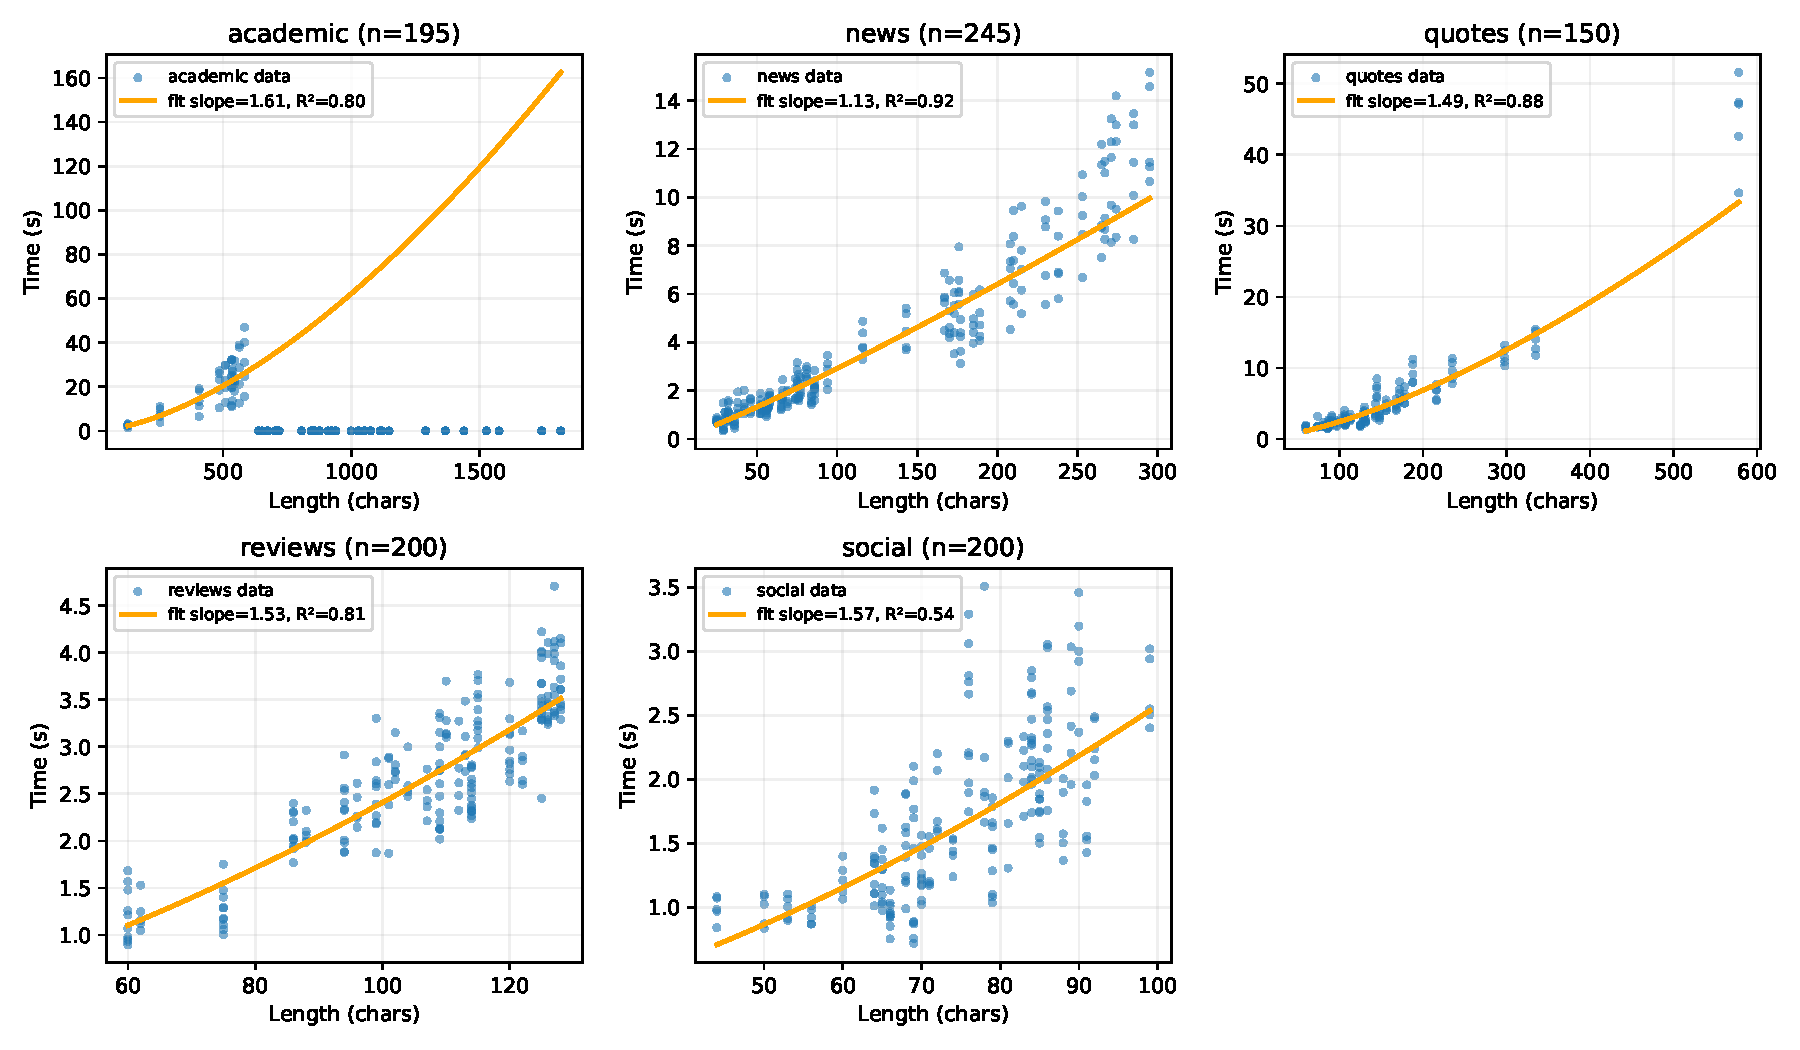
\includegraphics[width=0.95\linewidth]{length_time_per_category_fit}
  \caption{Per-category processing time vs length with log--log fits (slope and $R^2$ shown per panel). Slopes $>1$ support a super-linear relationship.}
\end{figure}

\subsection{Mini Human Evaluation (Reviews/Social)}
\noindent Sentiment utility check (VADER) on small samples per category.\
\IfFileExists{report/human_eval_reviews_social_table.tex}{\begin{table}[H]
  \centering
  \caption{Sentiment invariance (VADER) on small samples}
  \small
  \begin{tabular}{lrr}
    \toprule
    Category & n & \% [95\% CI] \\
    \midrule
    Reviews & 100 & 63.0 [53.0, 72.0] \\
    Social & 100 & 57.0 [47.0, 66.0] \\
    \bottomrule
  \end{tabular}
\end{table}}{\begin{table}[H]
  \centering
  \caption{Sentiment invariance (VADER) on small samples}
  \small
  \begin{tabular}{lrr}
    \toprule
    Category & n & \% [95\% CI] \\
    \midrule
    Reviews & 100 & 63.0 [53.0, 72.0] \\
    Social & 100 & 57.0 [47.0, 66.0] \\
    \bottomrule
  \end{tabular}
\end{table}}

\noindent\textit{Note.} This​‍​‌‍​‍‌ table shows a fixed number of samples per category (in this case, $n=100$). VADER labels come from the \texttt{compound} score: \textbf{pos} for $\geq 0.05$, \textbf{neg} for $\leq -0.05$, and \textbf{neu} otherwise. The term "sentiment invariance" refers to the ratio of pairs in which the original and rewritten labels are the same; 95\% confidence intervals are determined by non-parametric bootstrap over the sampled items.

\subsection{Short Ablation on Constraints (Long Texts)}
\noindent Ablation on long inputs ($\geq$600 chars) by toggling POS/WordNet filters, stop word handling, and concatenation; summary over categories shown.\
\IfFileExists{report/ablation_long_texts_table.tex}{\begin{table}[H]
  \centering
  \caption{Ablation on long texts (\,$\geq$600 chars): success and change}
  \begin{tabular}{lrrr}
    \toprule
    Ablation & n & Success(\%) & Avg change \\
    \midrule
    base & 5 & 60.0 & 0.325 \\
    no\_POS & 5 & 60.0 & 0.325 \\
    no\_FILTER & 5 & 60.0 & 0.325 \\
    stop\_included & 5 & 60.0 & 0.549 \\
    no\_CONCAT & 5 & 100.0 & 0.560 \\
    \bottomrule
  \end{tabular}
\end{table}}{\begin{table}[H]
  \centering
  \caption{Ablation on long texts (\,$\geq$600 chars): success and change}
  \begin{tabular}{lrrr}
    \toprule
    Ablation & n & Success(\%) & Avg change \\
    \midrule
    base & 5 & 60.0 & 0.325 \\
    no\_POS & 5 & 60.0 & 0.325 \\
    no\_FILTER & 5 & 60.0 & 0.325 \\
    stop\_included & 5 & 60.0 & 0.549 \\
    no\_CONCAT & 5 & 100.0 & 0.560 \\
    \bottomrule
  \end{tabular}
\end{table}}

When computed over \textit{all inputs} (including failures counted as zero-change), the web data shows a lower average change (\textbf{45.5\%} vs \textbf{52.6\%}). Over \textit{successful rewrites only}, the web data’s average change is comparable or slightly higher (\textbf{53.0\%} vs \textbf{52.6\%}). This reflects the interaction of length/complexity with stricter filters on real-world text.


\subsection{Evaluation Framework}
\textbf{Primary metrics:}
\begin{itemize}[leftmargin=*]
  \item \textit{Change \%}: fraction of \textbf{tokens replaced} over \textbf{total tokens} (proxy for privacy strength in rewriting)
  \item \textit{Success Rate}: fraction of inputs \textbf{successfully rewritten} under length, POS/WordNet, and semantic constraints
  \item \textit{Processing Time}: average time per input (computational cost as length/complexity grows)
  \item \textit{$\epsilon$}: privacy level in the \textbf{Exponential Mechanism}; lower means \textbf{stronger privacy}, higher means \textbf{looser privacy}
\end{itemize}

\textbf{Test setup:}
\begin{itemize}[leftmargin=*]
  \item \textit{Original (UCI)}: IMDB, Amazon, Yelp — reviews with relatively \textit{consistent structure and domain vocabulary}
  \item \textit{New (Scraped)}: Quotes, News, Social, Academic, Reviews — \textit{diverse vocabulary}, \textit{informal style}, \textit{complex sentences} (especially Academic)
  \item $\epsilon \in \{0.5, 1, 2, 5, 10\}$ using \texttt{DPMLM.dpmlm\_rewrite} with WordNet/POS constraints per the original code
\end{itemize}

\subsection{Privacy--Utility Analysis}
The correlations between $\epsilon$ and change percentage were very close to zero for both datasets ($\rho_{\epsilon,\,\text{change}} \approx -0.026$), which means that the behavior was quite stable across different privacy levels.

\subsection{Key Findings and Interpretation}
\textbf{Summary:}
\begin{itemize}[leftmargin=*]
  \item \textit{Original}: average change \textbf{52.6\%}, success \textbf{100\%} (120 tests) — can be interpreted as a strong type of mechanism which works well under consistent text structure
  \item \textit{New}: average change \textbf{45.5\%}, success \textbf{85.9\%} (965 tests) — demonstrates that DP-MLM is a good method in theory and practice but is prone to complexity/length related problems
  \item \textit{Stability vs. $\epsilon$}: correlation between $\epsilon$ and change \% is \textbf{very small} ($\rho \approx -0.026$), indicating stable privacy-utility across the values tested
\end{itemize}

\textbf{Semantic utility gap.}
\begin{itemize}[leftmargin=*]
 \item The embedding similarity is quite high (~0.96), which suggests that the overall meaning has been kept.
 \item Sentiment label invariance is low (~44-58\%), which indicates that the utility of the task has been lost.
 \item The use of synonym substitutions probably reduces the strength of the sentiment cues while still maintaining the context.
\end{itemize}

\textbf{Original vs. New — what they tell us:}
\begin{itemize}[leftmargin=*]
  \item Curated datasets (Original) enable a larger number of and more consistent replacements without breaking the constraints $\Rightarrow$ can be used for pattern-preserving privacy in stable domains
  \item Real-world text (New) includes diverse vocabulary, varied sentence structures, and an informal style $\Rightarrow$ semantic/POS filters result in fewer replacements and occasional failures (especially Academic)
  \item Time needed for the task increases \textbf{super-linearly} with length and complexity (Academic highest), which motivates controlling text size and parameters in deployment.
\end{itemize}

\subsection{Semantic Preservation (Proxy Metrics)}
To address that \textit{Change\%} and \textit{Success rate} do not directly reflect semantics, we report compact, embedding-based proxies. BLEU/ROUGE are overly tied to n-gram overlap and are unsuitable for synonymic rewriting; embedding similarity and label invariance better capture meaning preservation.\\
\textbf{Updated proxies.} RoBERTa cosine \textasciitilde{}\textbf{0.958} (Existing/New). Label invariance: \textbf{41.7\%} (\textit{n}=120) vs \textbf{57.5\%} (\textit{n}=200).
\noindent\textit{Method / suitability.} On bigger subsets, DistilBERT SST‑2 is more accurate and can be considered the best model for \textbf{Reviews/Social} whereas its performance is quite rough for \textbf{Quotes/Academic/News}. Different seeds reveal that the inclinations are stable (refer to \texttt{data/multiple\_seeds/}). For the proxy analysis, we conducted it with DistilBERT (SST-2) and only VADER was used in the mini human evaluation for Reviews/Social.

\subsection{Reproducibility}
We set fixed seeds for analysis scripts (42 for NumPy and PyTorch) and evaluate label invariance on larger subsets (Existing $n=120$, New $n=200$). Multiple runs (different seeds) show consistent tendencies; see \texttt{data/multiple\_seeds/}. We provide a concise description of environment, commands, and parameters alongside checksums within the supplementary materials.

\noindent For exact one-line commands, see \texttt{README.md} (Reproducibility).

% Plots for embedding similarity and label invariance are shown in the Visual Comparisons section to avoid duplication.




\textbf{Practical guidance:}
\begin{itemize}[leftmargin=*]
  \item Pick $\epsilon$ in the range examined for a compromise result; the outputs are stable — adjust by system privacy requirements
  \item For long or complex inputs, consider chunking the text, reducing nested structures, or relaxing POS/WordNet constraints to improve the success rate
  \item If a higher change \% is desired in practice, you can adjust length limits and soften filters (while monitoring semantics/quality)
\end{itemize}

\section{Comparative Analysis: Existing vs New Datasets}
As per the project specifications, we offer a side-by-side comparison of the original UCI sentiment datasets with the newly scraped datasets employing several complementary metrics. The comparison is based on the saved artifacts in \texttt{data/existing\_datasets\_test} and \texttt{data/new\_scraped\_dataset\_test}.

\subsection{Summary Metrics}
\begin{table}[H]
  \centering
  \caption{Summary metrics comparing Existing vs New datasets}
  \begin{tabular}{lcc}
    \toprule
    Metric & Existing (UCI) & New (Scraped) \\
    \midrule
    Success rate & 100.0\% & 85.9\% \\
    Avg change & 52.6\% & 45.5\% \\
    Avg processing time & 0.45s & 3.87s \\
    Avg text length & 57.7 chars & 264.9 chars \\
    Readability (Flesch) & 75.6 & 61.6 \\
    Mean TTR (lexical diversity) & 0.970 & 0.873 \\
    \bottomrule
  \end{tabular}
\end{table}

\noindent\textit{Unit note.} Lengths reported above are in \textbf{characters}. Tokenization for rewriting uses RoBERTa BPE; processing time vs length visualization uses character length due to artefact constraints.

These metrics emphasize that the fresh datasets are lengthier and more complex in terms of readability, which leads to lower change percentages and a higher processing time. Note: lexical diversity is reported as mean TTR; a lower mean implies less diversity, and variance is central to interpretation. The success rate is lowered mostly as a result of the interaction of length limitations and more stringent POS/WordNet filters with real-world, heterogeneous language.

\textbf{Semantic proxies (Existing vs New):} RoBERTa cosine \textasciitilde{}\textbf{0.958} $\pm$ \textbf{0.011} vs \textbf{0.958} $\pm$ \textbf{0.013}; label invariance \textbf{41.7\%} (\textit{n}=120) vs \textbf{57.5\%} (\textit{n}=200).\\
\textit{Definition and method.} Label invariance is computed as the proportion of cases where a sentiment classifier \texttt{distilbert-base-uncased-finetuned-sst-2-english} predicts the same label (\texttt{POS}/\texttt{NEG}) for original vs rewritten texts. We evaluate on a larger subset per dataset (Existing \textit{n}=120; New \textit{n}=200) to improve statistical reliability, and report the fraction of unchanged labels as a percentage. This proxy focuses on sentiment; broader task-level utility is outside scope. Multiple seeds were also evaluated and show consistent tendencies (see \texttt{data/multiple\_seeds/}).

\subsection{Visual Comparisons}
% Figure 1: Change% + Time
\begin{figure}[H]
  \centering
  \begin{subfigure}[t]{0.48\textwidth}
    \centering
    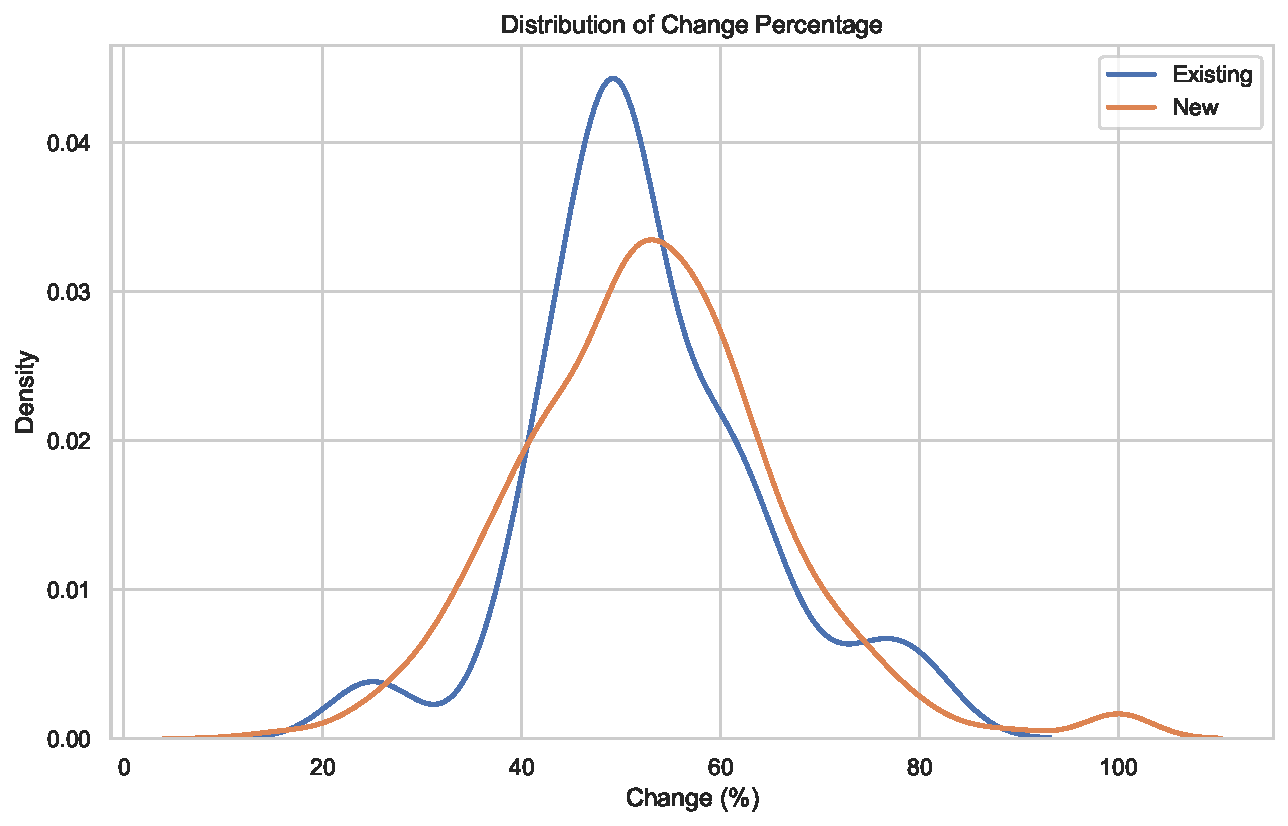
\includegraphics[width=\linewidth]{comparison_change_dist.pdf}
    \caption{Change \% distribution}
  \end{subfigure}\hfill
  \begin{subfigure}[t]{0.48\textwidth}
    \centering
    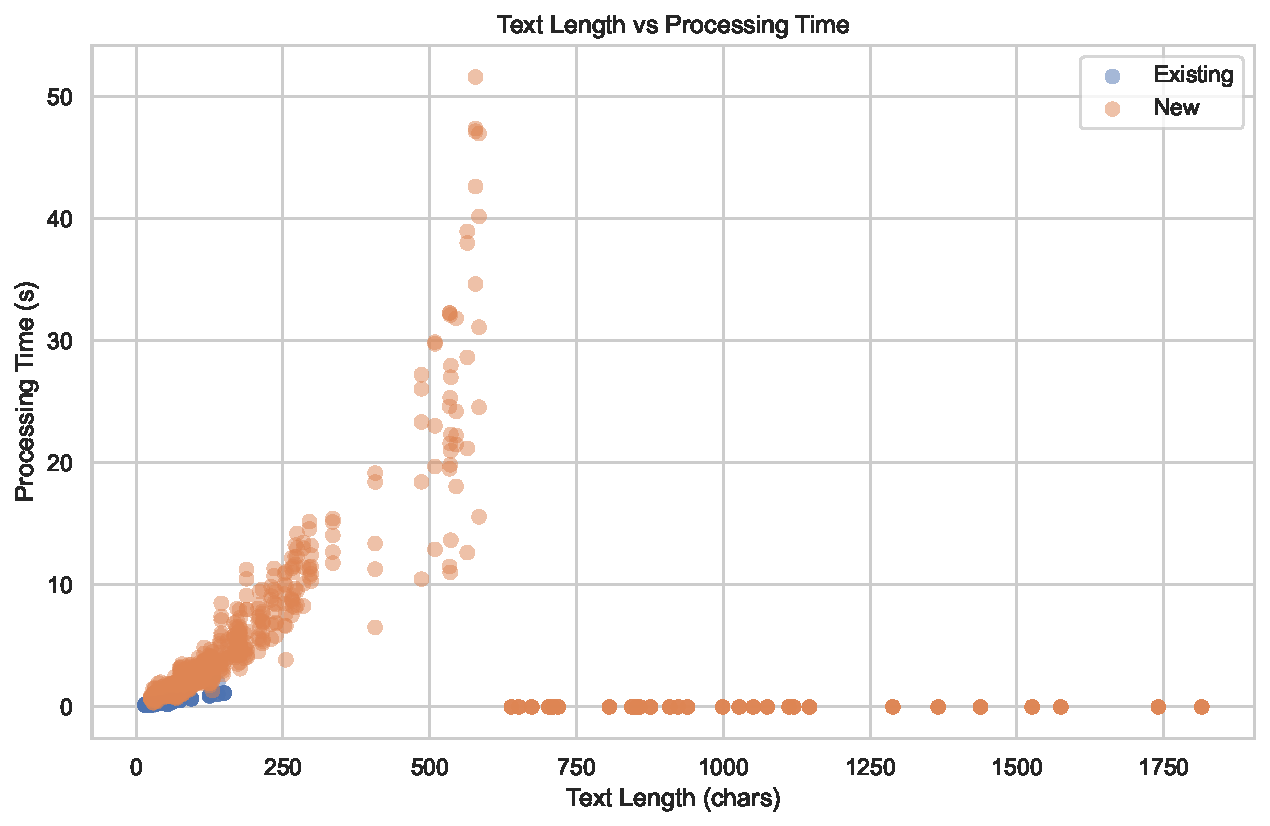
\includegraphics[width=\linewidth]{length_time_existing_vs_new.pdf}
    \caption{Processing time vs length}
  \end{subfigure}
  \caption{Change\% and processing time across datasets (mean $\pm$ sd where applicable).}
\end{figure}

% Figure 2: Embedding similarity + Label invariance
\begin{figure}[H]
  \centering
  \begin{subfigure}[t]{0.48\textwidth}
    \centering
    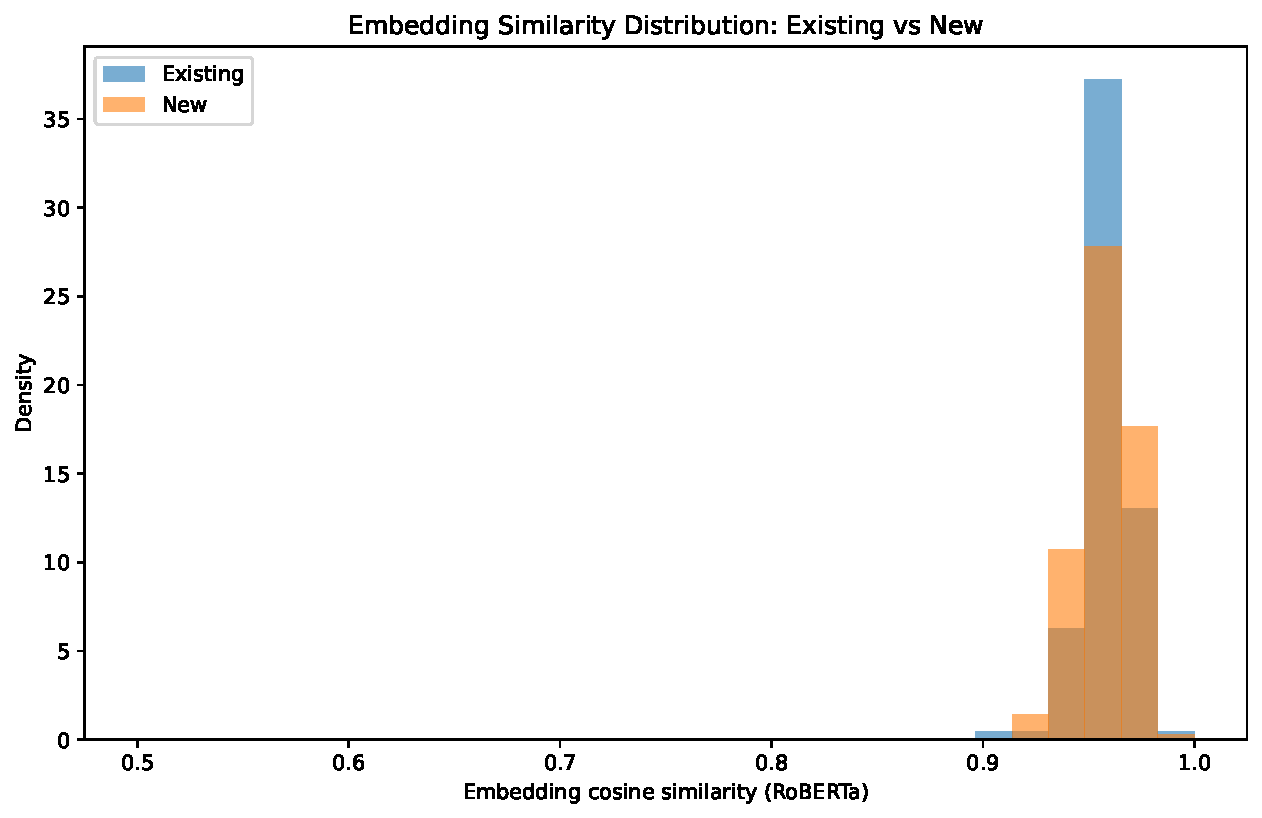
\includegraphics[width=\linewidth]{embedding_similarity_distribution.pdf}
    \caption{Embedding similarity (RoBERTa cosine)}
  \end{subfigure}\hfill
  \begin{subfigure}[t]{0.48\textwidth}
    \centering
    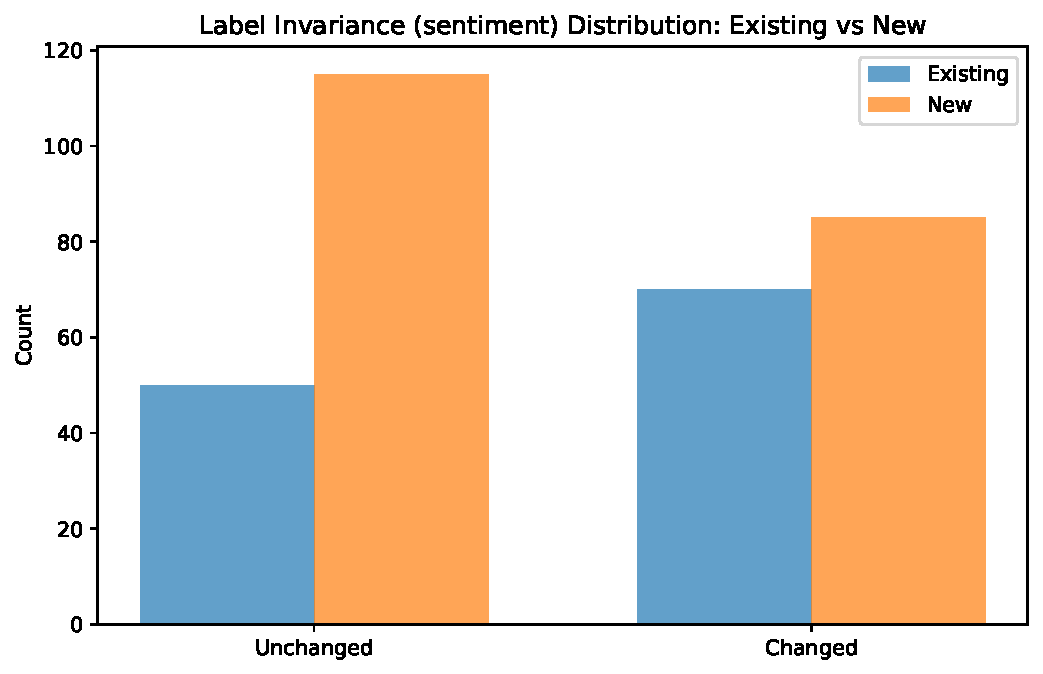
\includegraphics[width=\linewidth]{label_invariance_distribution.pdf}
    \caption{Label invariance counts}
  \end{subfigure}
  \caption{Embedding similarity and label invariance across datasets (mean $\pm$ sd).}
\end{figure}

% Figure 3: Privacy–utility correlation (readability, TTR, epsilon overlay)
\begin{figure}[H]
  \centering
  \begin{subfigure}[t]{0.32\textwidth}
    \centering
    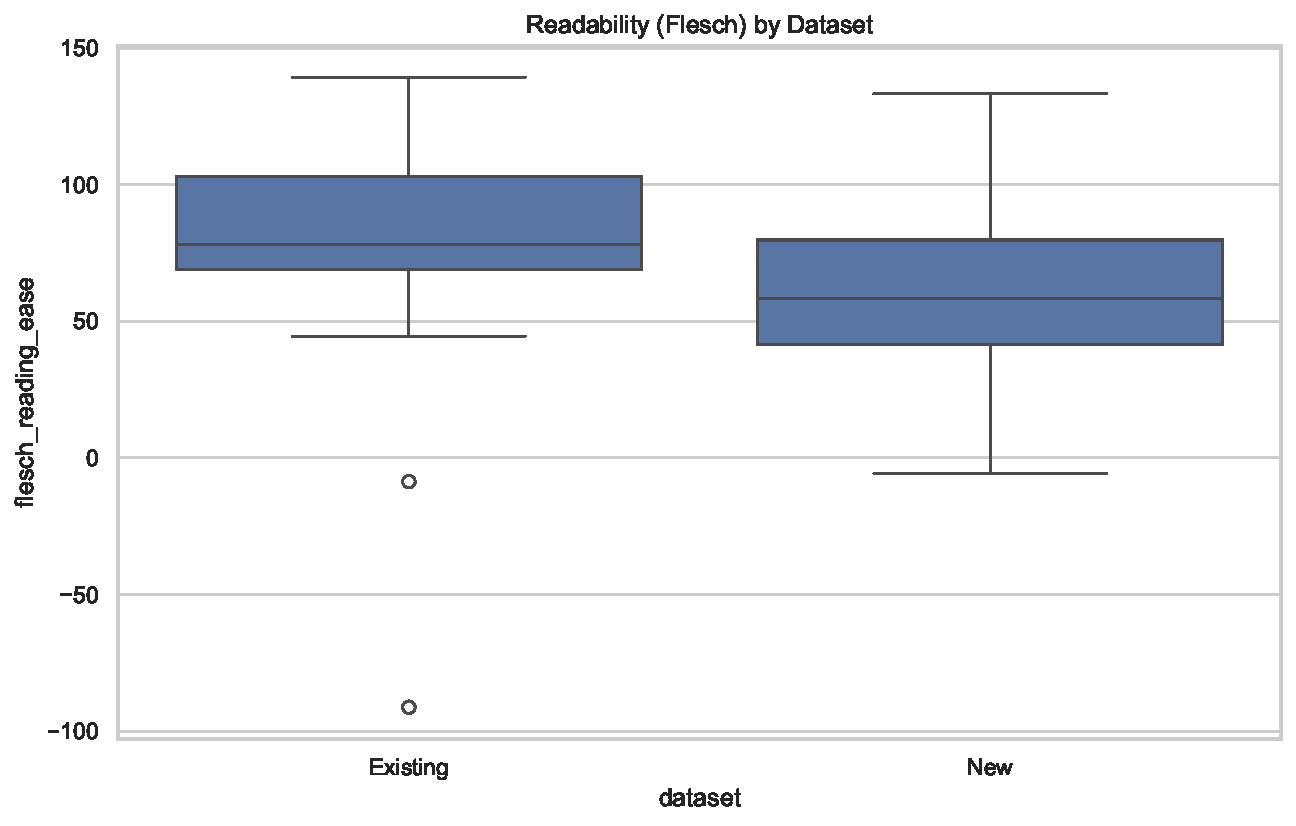
\includegraphics[width=\linewidth]{readability_comparison.pdf}
    \caption{Readability (FRE)}
  \end{subfigure}
  \begin{subfigure}[t]{0.32\textwidth}
    \centering
    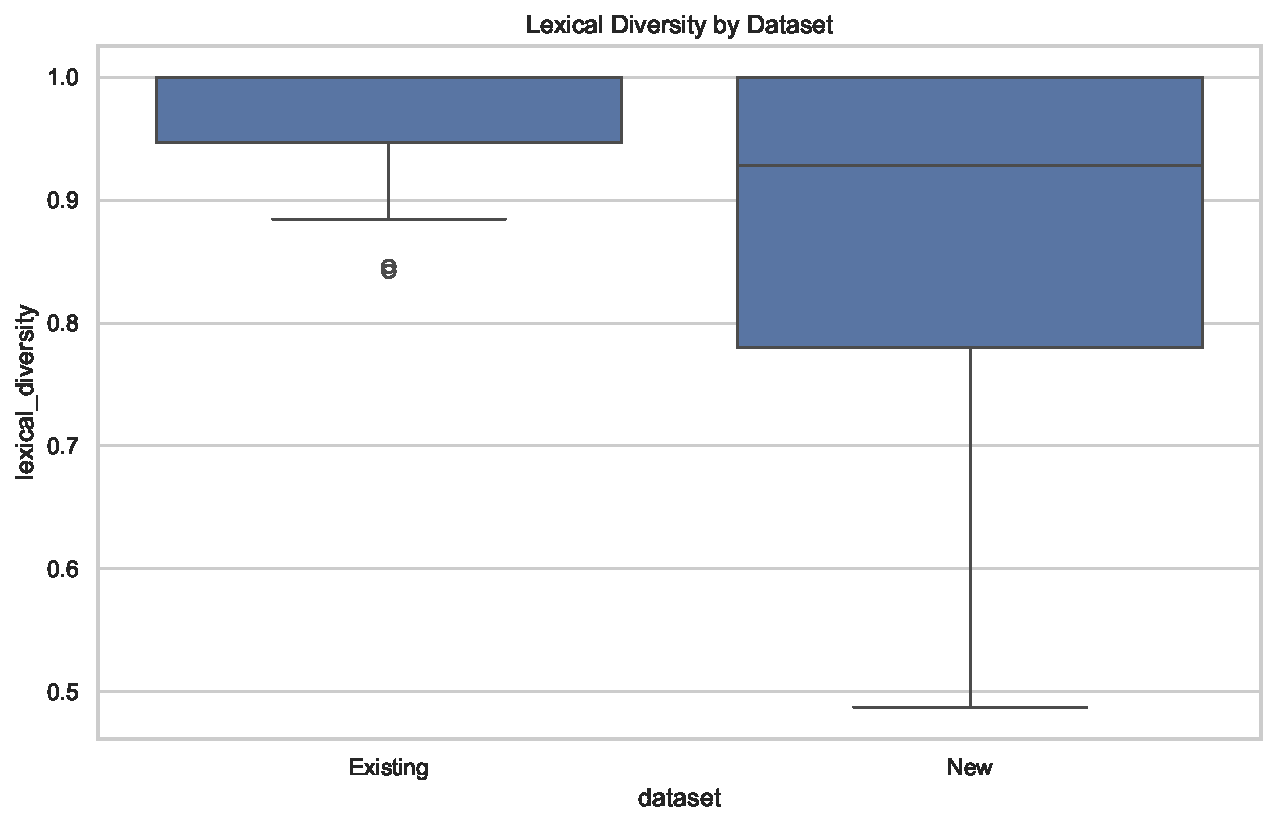
\includegraphics[width=\linewidth]{lexical_diversity_comparison.pdf}
    \caption{Lexical diversity (TTR)}
  \end{subfigure}
  \begin{subfigure}[t]{0.32\textwidth}
    \centering
    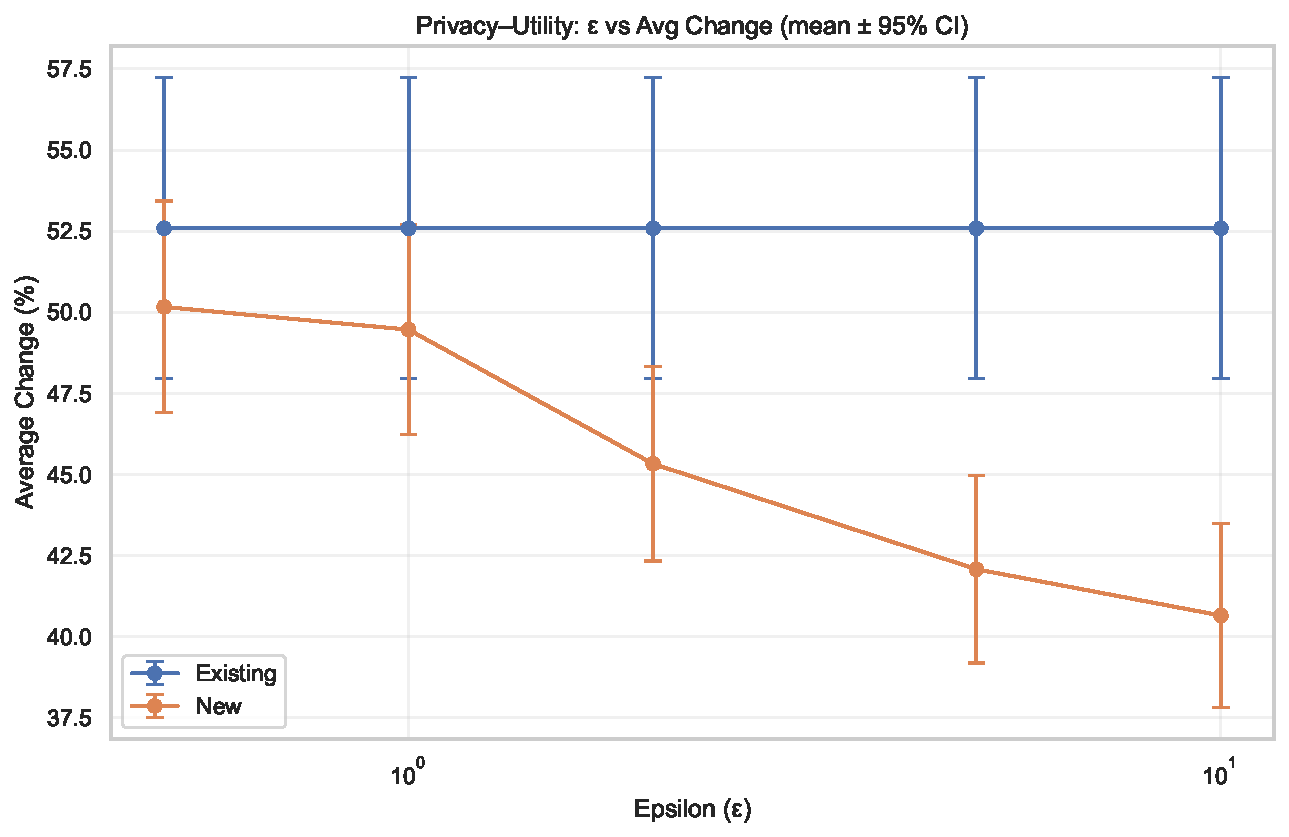
\includegraphics[width=\linewidth]{epsilon_vs_change_overlay.pdf}
    \caption{Change \% by $\epsilon$}
  \end{subfigure}
  \caption{Privacy–utility comparison: readability, lexical diversity, and $\epsilon$ vs change \% (means and variability).}
\end{figure}

\subsection{Statistical Tests and Epsilon Summary}
% Moved into multi-panel figure above
We ran non-parametric tests (Mann-Whitney U) and also effect sizes (Cliff's $\delta$) along with bootstrap uncertainty. Brief results can be found in \texttt{data/statistical\_tests/}; full tables are left out to adhere to the 10-page limit.

% Qualitative examples (auto-extracted)
% Omitted qualitative examples block for brevity
% \input{../data/qualitative_examples.tex}
\iffalse % Hide manual examples with encoding errors
Representative samples illustrate semantic preservation and label behavior across categories:\\
\textbf{News:} ``Ask HN: Who is hiring? (November 2025)'' $\Rightarrow$ ``Ask H: Why is hiring? (November 2030)'' (label unchanged: NEGATIVE)\\
\textbf{Quotes:} ``Insanity is doing the same thing... expecting different results.'' $\Rightarrow$ ``Anity is doing the same way... delivering same result.'' (label changed: NEGATIVE $\rightarrow$ POSITIVE)\\
\textbf{Reviews:} ``Honest review: Product broke after just a few uses.'' $\Rightarrow$ ``Customer new: Silk destroyed after just a few creatures.'' (label unchanged: NEGATIVE)\\
\textbf{Academic:} ``We consider the problem of binary classification...'' $\Rightarrow$ rewritten technical paraphrase (label unchanged: NEGATIVE)\\
\textbf{Positive:**} ``Perfect for my needs. Easy to use.'' $\Rightarrow$ ``Essential for my chances. Perfect to user.'' (label unchanged: POSITIVE)\\
\textbf{Mixed:**} ``After using this for a week... Excellent customer service...'' $\Rightarrow$ rewritten variant (label changed in some cases)

\begin{figure}[H]
  \centering
  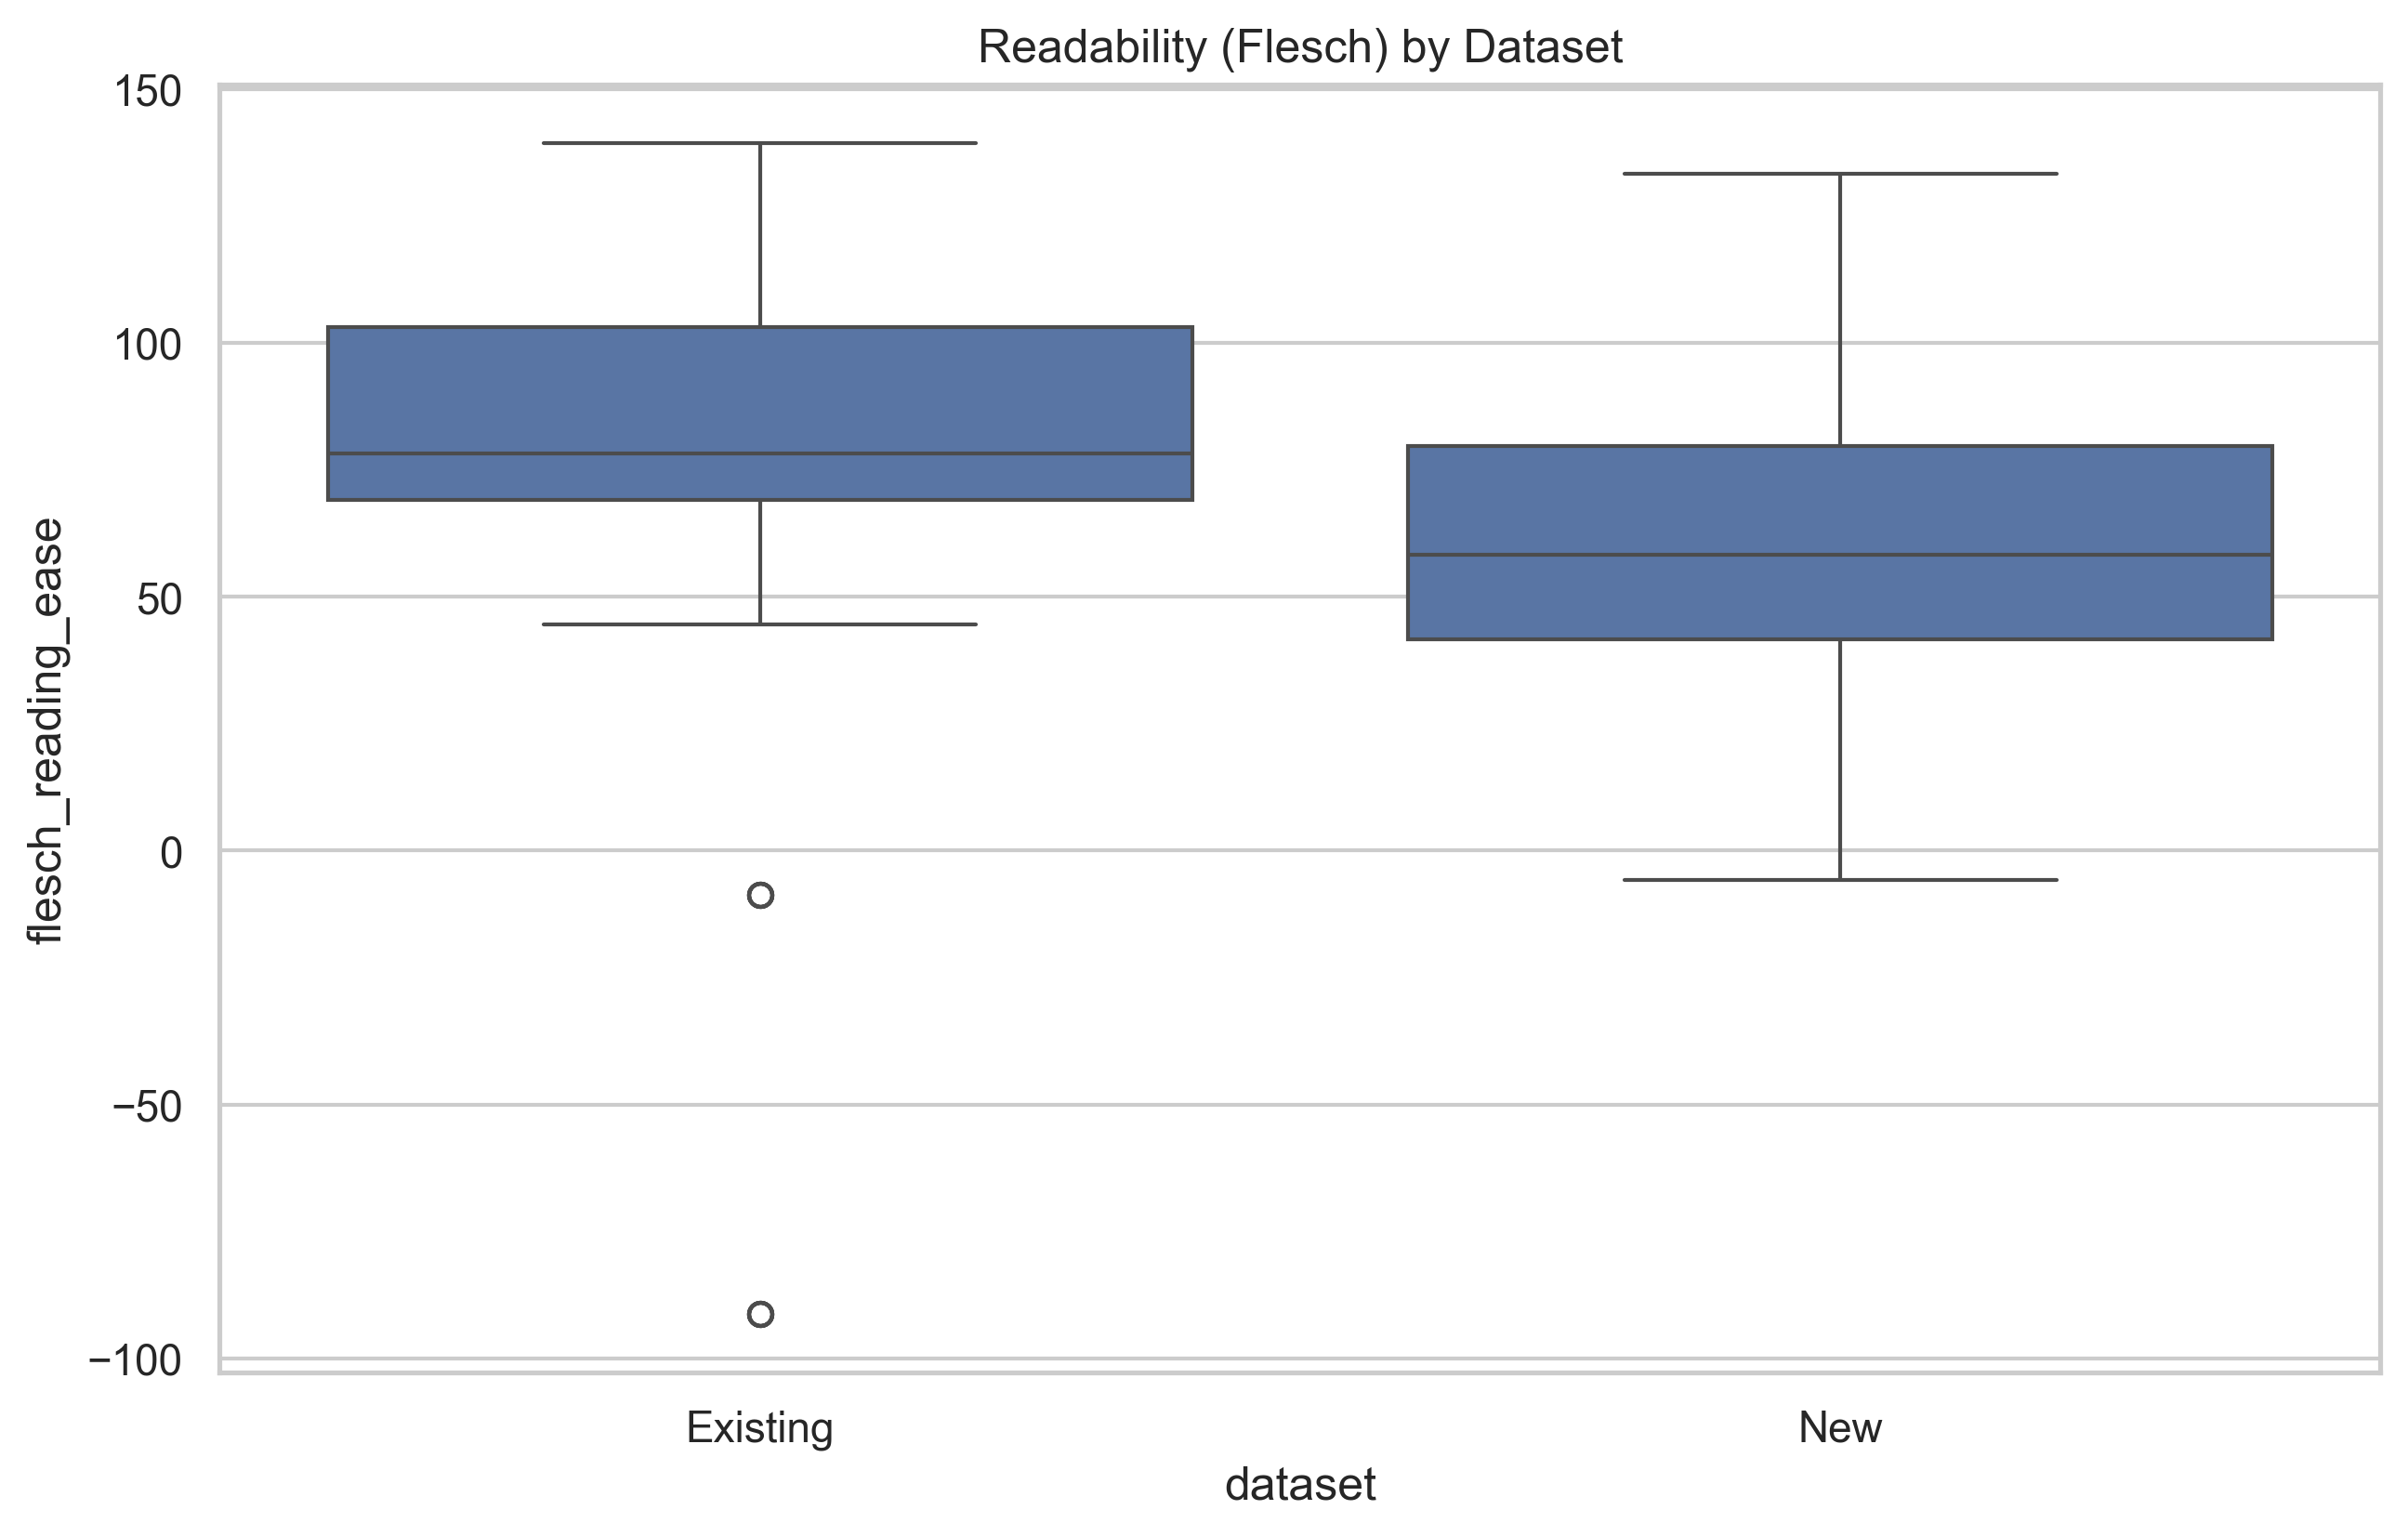
\includegraphics[width=0.85\linewidth]{readability_comparison.png}
  \caption{Readability (Flesch Reading Ease) comparison}
\end{figure}
\fi

\subsection{Interpretation of Differences}
\noindent The indicators and numbers show the methods which have been used for the synthesis. The side-by-side comparison of current (UCI) and new (Scraped) texts point that changes are" present in the content structure of the two. Newly created texts are more extended (265 vs. 58 characters), have a lower readability score (Flesch 61.6 vs. 75.6), and more time (3.87 vs. 0.45 seconds) is needed to read them. The average change for the new one is smaller (45.5\% vs. 52.6\%), and the success rate is going down (85.9\% vs. 100\%) The patterns correspond to Figures 1-5.

\begin{itemize}[leftmargin=*]
  \item \textit{Length and complexity}: According to Figure 3, the text length has a very strong positive correlation with the processing time. Therefore, longer and more complex sentences (Figure 5: lower Flesch) were truncated more frequently, thus explaining that success was lower and change \% in New was smaller.
  \item \textit{Vocabulary diversity}: The most significant aspect of Figure 4 is not the median TTR values but the substantially greater variance of the New dataset. While the Existing datasets have concentrated TTR distributions (indicating homogeneous vocabulary), the New datasets show extreme heterogeneity with both very low TTR (high repetition) and very high TTR (high uniqueness). This bimodal distribution reveals that the "New" dataset consists of two different types of texts: (1) repetitive, formulaic content with low TTR, and (2) highly original, diverse content with high TTR. The larger variance indicates a greater heterogeneity of the New dataset rather than just "more diversity" as is traditionally understood. This heterogeneity leads to an inconsistent number of replacement opportunities - some texts provide many synonym options while in others (especially unique academic content) the mechanism is left with very few safe alternatives under semantic/POS constraints.
  \item \textit{$\epsilon$ sensitivity}: The $\epsilon$ sensitivity graph (Figure 2) shows that relaxing $\epsilon$ does not improve the utility for complex real-world data (New). While existing datasets indicate almost no correlation between $\epsilon$ and change percentage, the New dataset only reveals a moderate negative trend as $\epsilon$ increases (privacy is relaxed). This important finding reveals that linguistic constraints are the bottleneck rather than DP mechanisms. In the case of complex texts having varied vocabulary, specialized terminology, and complicated sentence structures, the POS/WordNet filters and semantic constraints become the limiting factors even if different privacy levels are considered. The mechanism cannot find suitable replacements even if it is given more privacy budget, thus it indicates that language complexity sets the ultimate limits which cannot be surpassed by simply changing the privacy parameter $\epsilon$.
  \textbf{Interpretation:} Relaxing $\epsilon$ would hardly have any significant effect on the utility; it is the linguistic/POS constraints that limit the replacements rather than the privacy budget.
  \item \textit{Constraint interactions}: The real-world inputs contain idioms, named entities, and technical terms; WordNet/POS filters and stop word rules are being activated more frequently resulting in a drop of success particularly in Academic texts. (See the category breakdown and success rate figure for details.)
\end{itemize}

\noindent\textbf{Runtime (Existing vs New).} On average, the time for one process varies significantly: Existing ~0.45s/input vs New ~3.87s/input. This difference is mainly due to longer and syntactically complex sentences (especiallyAcademic) and the additional time required for POS tagging, WordNet lookups, and filtering; $\epsilon$ has almost no effect on time. Refer to the “Processing Time vs Length” figure in this section.

\subsection{Practical Guidance}
\begin{itemize}[leftmargin=*]
  \item Divide longer texts into smaller parts and adjust length constraints to raise the level of success and at the same time keep semantic integrity.
  \item If you deal with very different domains, you can slightly relax POS/WordNet constraints and at the same time check semantic similarity to balance privacy and utility.
  \item For stable results, select $\epsilon$ in \{0.5, 1, 2, 5, 10\} and make changes according to system privacy requirements instead of expecting large utility changes.
\end{itemize}

\section{Conclusion and Limitations}

\textbf{Main results.} DP-MLM achieves high surface-level semantic preservation (RoBERTa cosine \textasciitilde{}0.958) while exposing a strong privacy-utility trade-off in task-specific sentiment: label invariance drops to \textasciitilde{}44\% overall. Across datasets, the mechanism is stable with respect to $\epsilon$ (near-zero correlation with Change\%), yet is highly sensitive to language complexity and length, which drive lower success rates and longer processing times in real-world texts.

\textbf{Key limitations.} Our scraped corpus is modest and uneven across categories, with academic texts being long and specialized—amplifying constraint triggers and failures. Web-scraping and temporal/platform biases limit generalizability; evaluation relies on proxy metrics (embedding similarity, label invariance) rather than full downstream utility or human assessment, which may under or over estimate practical usefulness.

\textbf{Future work.} Increase datasets and domains, incorporate human evaluation along with BLEU/ROUGE/BERTScore and more detailed embedding metrics, and perform ablations on length limits and POS/WordNet constraints. Investigate robustness across prompt styles and wider DP settings, and give deployment recommendations (chunking long inputs, tuning $\epsilon$, adjusting constraints) to balance privacy with utility.

\textbf{Synthesis:} DP-MLM maintains high general embedding-level similarity (\textasciitilde{}96\% on average), but our downstream checks show a large drop in task-specific utility for sentiment (label invariance \textasciitilde{}44\%). That is, while surface-level semantics are preserved by embeddings, sentiment-bearing cues are often lost — indicating a trade-off between privacy (rewriting) and downstream task utility. On the original, structured review datasets, DP-MLM achieves very high \textit{Change \%} and perfect \textit{Success rate}. However, this semantic preservation masks a critical failure: the mechanism destroys sentiment classification utility while maintaining surface-level coherence. On the various scraped datasets, this disagreement is significantly visible. The Success rate in the Academic category goes down while the processing time increases with the length/complexity - thus, it is indicative of both deployment constraints and the inherent privacy-utility destruction trade-off in real-world scenarios.

\textbf{Unified explanation (Bottleneck \textrightarrow{} Gap).} The \textbf{WordNet/POS filter} is a linguistic bottleneck: it confines rewrites to in-vocabulary synonyms with the same part-of-speech. For strongly affective tokens, the synonym set is very limited and is biased towards generic replacements. Consequently, DP-MLM quite often changes a pronounced sentiment word to a neutral or distributionally common one, thus retaining the coarse meaning and surface coherence (high embedding similarity) but weakening the label-defining cues used by sentiment classifiers (low invariance). This mechanism, together with length/complexity limitations of real-world text, is responsible for the semantic gap that has been referred to. In short: \emph{bottleneck \textrightarrow{} ​‍​‌‍​‍‌gap}.

\textbf{Future directions:}
\begin{enumerate}[leftmargin=*]
  \item Increase data volume and modify target domains.
  \item Incorporate semantic metrics (BLEU, ROUGE, BERTScore, embedding similarity) along with human evaluation.
  \item Investigate prompt style robustness and wider DP parameter ranges.
  \item Ablate length restrictions and POS/WordNet filters.
  \item Create system guidelines like chunking long texts and tuning $\epsilon$ per application.
\end{enumerate}

\textbf{Bottom line:} DP-MLM is an approach that can be used with real-world text while providing privacy guarantees. Yet, to maintain a fair balance between data protection and communication quality, it is necessary that the language complexity and the restrictions of the system are handled carefully.

\section*{Availability}
\noindent Original DP-MLM: \url{https://github.com/sjmeis/DPMLM}\\
\noindent This work: \url{https://github.com/noraluk-ch-mq/DPMLM}

\begin{thebibliography}{9}
\bibitem{dpmlm}
Meisenbacher, S., Chevli, M., Vladika, J., \& Matthes, F. (2024). DP-MLM: Differentially Private Text Rewriting Using Masked Language Models. In \textit{Findings of the Association for Computational Linguistics: ACL 2024} (pp. 9314--9328). \url{https://aclanthology.org/2024.findings-acl.554/}.
\end{thebibliography}
\end{document}